\documentclass[tikz,border=6pt]{standalone}
\usepackage{pgfplots}
\pgfplotsset{compat=1.18}
\usepgfplotslibrary{colormaps}
\usetikzlibrary{arrows, arrows.meta, calc}
\usetikzlibrary{decorations.markings}


\usepackage{amssymb,amsmath,mathtools}

\usepackage[T1]{fontenc}
\usepackage[utf8]{inputenc}
\usepackage{newpxtext,newpxmath}
\usepackage{sectsty}

\renewcommand{\Re}{\operatorname{\mathrm{Re}}}
\renewcommand{\Im}{\operatorname{\mathrm{Im}}}

\begin{document}
	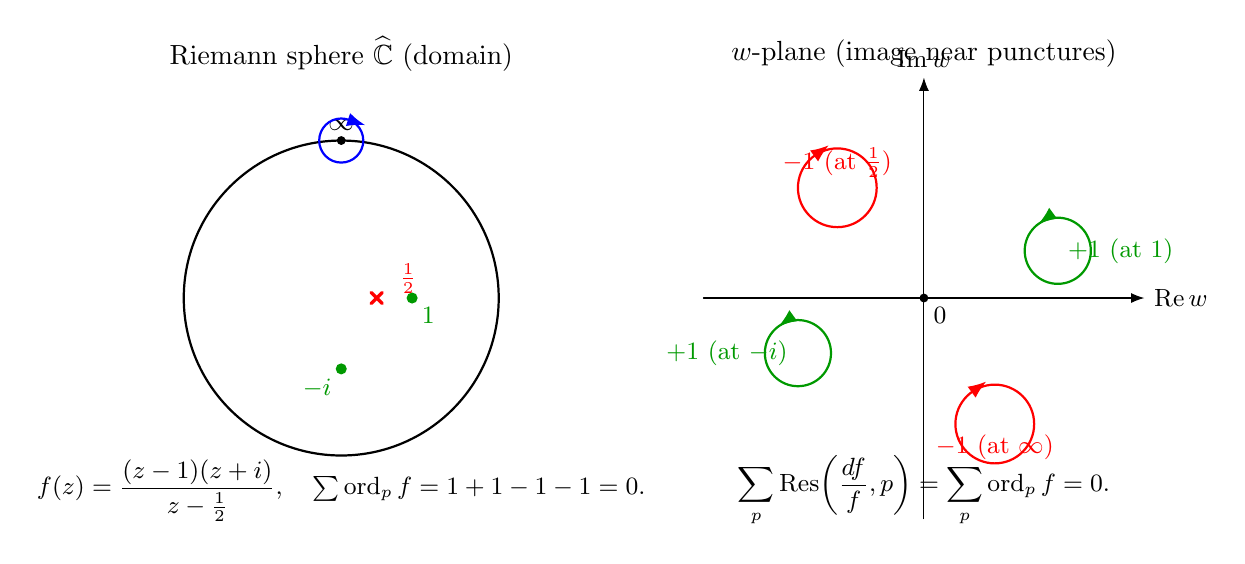
\begin{tikzpicture}[>=Latex, line cap=round, line join=round, font=\small]
		
		% ===== Left: Riemann sphere with punctures (zeros/poles incl. infinity) =====
		\begin{scope}
			\node[font=\normalsize] at (0,3.1) {Riemann sphere $\widehat{\mathbb C}$ (domain)};
			% sphere silhouette
			\draw[thick] (0,0) circle (2.0);
			% mark points: zeros (green), finite pole (red), infinity pole (red)
			% zeros
			\fill[green!60!black] (0.9,0) circle(2pt) node[below right] {$1$};
			\fill[green!60!black] (0,-0.9) circle(2pt) node[below left] {$-i$};
			% finite pole
			\draw[red,very thick] (0.45,0) ++(-0.07,-0.07) -- ++(0.14,0.14);
			\draw[red,very thick] (0.45,0) ++(-0.07,0.07)  -- ++(0.14,-0.14);
			\node[red] at (0.85,0.25) {$\tfrac12$};
			% infinity as a pole: small clockwise boundary near top
			\fill (0,2.0) circle(1.6pt) node[above] {$\infty$};
			\draw[blue,thick,postaction={decorate},
			decoration={markings, mark=at position 0.2 with {\arrow{<}}}]
			(0,2.0) circle (0.28);
			
			% small circles around finite punctures (clockwise orientation)
%			\foreach \P in {(0.9,0),(0,-0.9),(0.45,0)}{
%				\draw[blue,thick,postaction={decorate},
%				decoration={markings, mark=at position 0.2 with {\arrow{<}}}] (\P) circle (0.25);
%			}
			
			\node at (0,-2.45) {$f(z)=\dfrac{(z-1)(z+i)}{\,z-\tfrac12\,},\quad
				\sum \operatorname{ord}_p f = 1+1-1-1=0.$};
		\end{scope}
		
		% ===== Right: w-plane image: local loops about 0 with signs =====
		\begin{scope}[shift={(7.4,0)}]
			\node[font=\normalsize] at (0,3.1) {$w$-plane (image near punctures)};
			\draw[->] (-2.8,0)--(2.8,0) node[right] {$\Re w$};
			\draw[->] (0,-2.8)--(0,2.8) node[above] {$\Im w$};
			\fill (0,0) circle(1.6pt) node[below right] {$0$};
			
			% zeros -> CCW loops (contrib +1 each)
			\draw[green!60!black,thick,postaction={decorate},
			decoration={markings, mark=at position 0.35 with {\arrow{>}}}]
			(1.7,0.6) circle (0.42) node[right] {+1 (at $1$)};
			\draw[green!60!black,thick,postaction={decorate},
			decoration={markings, mark=at position 0.35 with {\arrow{>}}}]
			(-1.6,-0.7) circle (0.42) node[left] {+1 (at $-i$)};
			
			% finite pole -> CW loop (contrib -1)
			\draw[red,thick,postaction={decorate},
			decoration={markings, mark=at position 0.35 with {\arrow{<}}}]
			(-1.1,1.4) circle (0.5) node[above] {$-1$ (at $\tfrac12$)};
			
			% pole at infinity -> CW loop (contrib -1)
			\draw[red,thick,postaction={decorate},
			decoration={markings, mark=at position 0.35 with {\arrow{<}}}]
			(0.9,-1.6) circle (0.5) node[below] {$-1$ (at $\infty$)};
			
			\node[align=center] at (0,-2.45)
			{$\displaystyle \sum_p \operatorname{Res}\!\left(\frac{df}{f},p\right)
				= \sum_p \operatorname{ord}_p f = 0.$};
		\end{scope}
		
	\end{tikzpicture}
\end{document}
